\subsection*{2.ii}

El siguiente \textbf{modelo E-R corresponde} a una base de datos de \textbf{una universidad}. Luego de unos años de funcionamiento, se han detectado una \textbf{serie de deficiencias en el sistema de mantenimiento} de datos y se quieren realizar las \textbf{siguientes modificaciones}:
\begin{figure}[H]
    \centering
    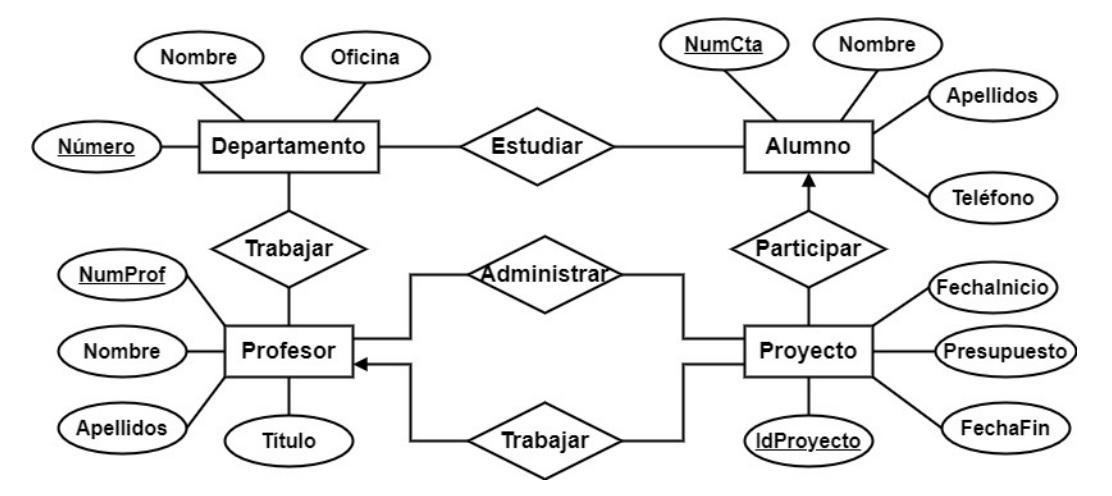
\includegraphics[width=1\linewidth]{imagenes/ModeloOriginal.png}
\end{figure}
\begin{itemize}
    \item Dado que solo los alumnos graduados pueden participar en proyectos, se desea distinguir entre alumnos graduados y no graduados. Además de la información almacenada para un alumno, para los alumnos graduados se desea almacenar el título que posee y para los alumnos no graduados su número de expediente.
    \item Un alumno graduado puede ser tutor de varios alumnos no graduados y cada alumno no graduado tendrá solamente un tutor.
    \item Se desea almacenar, para cada profesor, el nombre del cargo que ocupa en cada departamento (el cual es único dentro del departamento) y la carga horaria asociada. Un mismo cargo puede tener diferente carga horaria dependiendo del departamento y/o del profesor. Dentro de un departamento no pueden existir profesores con el mismo cargo. Un profesor podrá tener el mismo cargo en varios departamentos.
    \item Cuando un alumno graduado participa en un proyecto y un profesor debe supervisar su trabajo en ese proyecto. Cada alumno graduado podrá trabajar en múltiples proyectos, en los cuales podrá ser supervisado por diferentes profesores.
\end{itemize}
\textbf{Obtén un nuevo modelo E-R modificando el modelo presentado, para incorporar los cambios deseados. Identifica las restricciones de cardinalidad, participación e identidad en el nuevo modelo propuesto.}\\ 
\begin{figure}[H]
        \centering
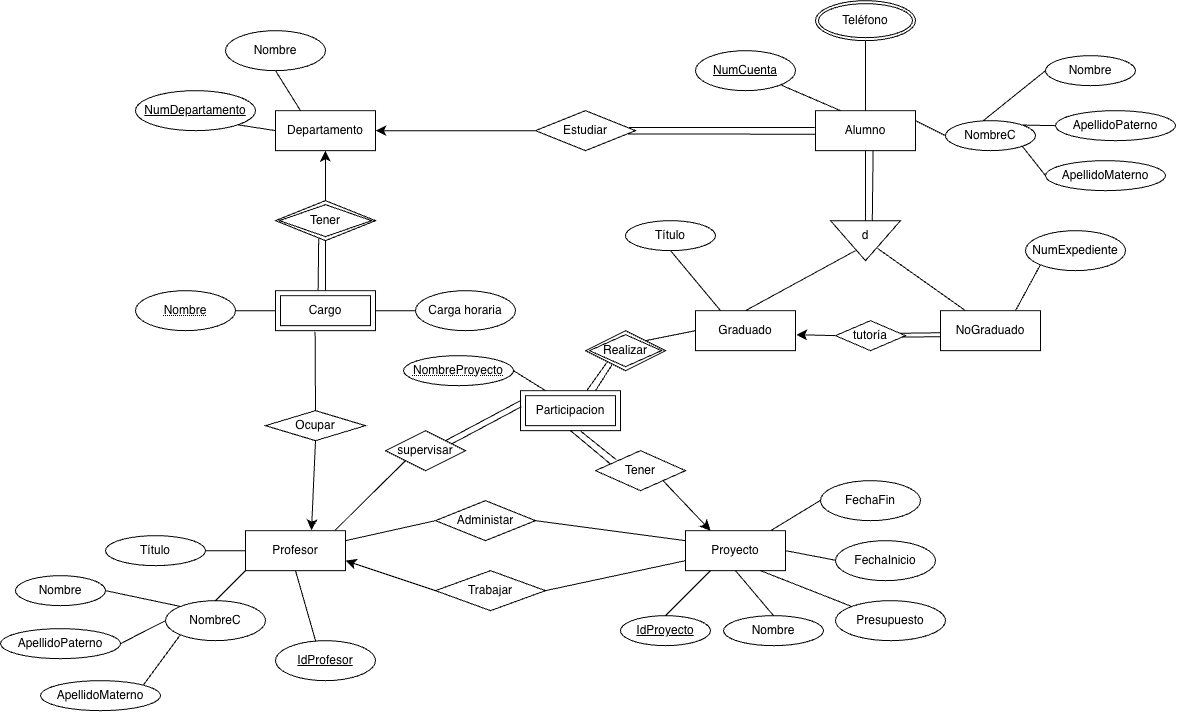
\includegraphics[width=1.1\linewidth]{imagenes/ModeloModificado.png}
    \end{figure}

\subsubsection*{Entidades:}
\begin{itemize}
    \item Profesor
    \item Departamento
    \item Proyecto
    \item Participación(Débil)
    \item Cargo(Débil)
    \item Alumno (SuperEntidad)
    \begin{itemize}
        \item Graduado
        \item No Graduado
    \end{itemize}
\end{itemize}
\subsubsection*{Atributos:}
\textbf{Profesor}
\begin{itemize}
    \item Titulo
    \item Nombre Completo(Nombre,Paterno,Materno)
    \item IdProfesor(identificador)
\end{itemize}
\textbf{Departamento}
\begin{itemize}
    \item Nombre 
    \item Número de Departamento(identificador)
\end{itemize}
\textbf{Proyecto}
\begin{itemize}
    \item Fecha de Inicio
    \item Fecha de Fin
    \item Presupuesto
    \item IdProyecto(identificador)
\end{itemize}
\textbf{Participación}
\begin{itemize}
    \item Nombre del proyecto(discriminante)
\end{itemize}
\textbf{Cargo}
\begin{itemize}
    \item Nombre del cargo(discriminante)
    \item carga horaria
\end{itemize}
\textbf{Alumno}
\begin{itemize}
    \item Telefono(multivaluado)
    \item Nombre Completo (Nombre,Paterno,Materno)
    \item Número de cuenta (identificador)
\end{itemize}
\textbf{Graduado}
\begin{itemize}
    \item Titulo
\end{itemize}
\textbf{No Graduado}
\begin{itemize}
    \item Número de expediente
\end{itemize}

\subsubsection*{Relaciones:}
\begin{itemize}
    \item \textbf{Estudiar} Departamento-Alumno \textbf{1:N}\\ \\
    Departamento: Parcial(0,N)\\
    Alumno:Total(1,1)\\ \\
    Muchos alumnos estudian en un  departamento. \\ \\
    Un alumno necesita estudiar en un departamento. \\
     
    \item \textbf{Tutoria} Graduado-NoGraduado \textbf{1:N}\\ \\
    Graduado:Parcial(0,N)\\
    No Graduado:Total(1,1)\\ \\
    Un alumno graduado puede ser tutor de varios alumnos no graduados. \\ \\
    Los alumnos no graduados solo tienen 1 tutor.

    \item \textbf{Realizar} Graduado-Participación \textbf{1:N}\\ \\
    Graduado:Parcial(0,N)\\
    Participación:Total(1,1)\\

    Los alumos pueden realizar varias participaciones en distintos proyectos.\\ \\
    Una participacion requiere necesariamente un alumno

\item \textbf{Tener} Proyecto-Participación \textbf{1:N}\\ \\
    Proyecto:Parcial(0,N)\\
    Participación:Total(1,1)\\ \\
    Una participación requiere necesariamente un proyecto.\\ \\
    Un proyecto puede tener varias participaciones de alumnos.
 
    \item \textbf{Supervisar} Profesor-Participación \textbf{N:M}\\ \\
    Profesor:Parcial(0,N)\\
    Participación:Total(1,M)\\ \\
Cada participacion puede ser supervisada por varios profesores.\\ \\
Un profesor puede supervisar varias participaciones.

    \item \textbf{Ocupar} Profesor-Cargo \textbf{1:M}\\ \\
    Profesor:Parcial(0,N)\\
    Cargo:Total(1,1)\\ 
    
    Los profesor pueden tener varios cargos en distintos departamentos.

    \item \textbf{Tener} Departamento-Cargo \textbf{1:M}\\ \\
    Departamento:Parcial(0,N)\\
    Cargo:Total(1,1)\\ \\
    Dentro de un departamento no pueden existir alguien con el mismo cargo.\\ \\
    Un cargo necesita estar asociado a un departamento.

    \item \textbf{Trabajar} Profesor-Proyecto \textbf{1:N}\\ \\
    Profesor:Parcial(1,N)\\
        Proyecto:Parcial(1,M)\\
    
    Muchos profesores administran varios proyectos
    \item \textbf{Administrar} Profesor-Proyecto \textbf{N:M}\\ \\
    Profesor:Parcial(0,N)\\
    Proyecto:Parcial(1,M)\\ 
    Los profesor pueden administrar varios proyectos.\\ \\
    Un proyecto puede ser administrado por varios profesores.
\end{itemize}